\documentclass[../main.tex]{subfiles}
\begin{document}
\newpage
\section{Вычисление объемов.}
\emph{Объём} - неотрицательная функция множества, определённая на некотором наборе множеств \( \mathcal{T}\), которые называются \emph{кубируемыми}. 
\[ A,B\in\mathcal{T} \implies A \cup B\in\mathcal{T},\; A\backslash B\in\mathcal{T},\; B\backslash A\in\mathcal{T},\;A \cap B\in\mathcal{T}\]
\begin{prop}{Свойства объёма:}
    Здесь всё по аналогии с площадью.
    \begin{enumerate}
        \item \emph{Аддитивность}\\
        \[T_1, T_2\in\mathcal{T},\quad T_1 \cap T_2= \varnothing \implies V\left( T_1 \cup T_2\right)=V\left( T_1\right)+V\left( T_2\right)\]
        \item \emph{Инвариантность относительно \hyperlink{def:movement}{изометрий}}\\
        \[ T\in\mathcal{T},\quad \Phi:\R^3 \longrightarrow \R^3\text{ - \hyperlink{def:movement}{изометрия}} \implies \Phi\left( T\right)\in\mathcal{T},\quad V\left( \Phi\left( T\right)\right)=V\left( T\right)\]
        \item \emph{Нормированность} \\
        Если \( Q\) - прямоугольный параллелепипед со сторонами \( a,b,c\), то \( Q\in\mathcal{T},\quad V\left( Q\right)=abc\).\\ 
        Если при этом одно из чисел \( a,b,c =0\), то параллелепипед называется вырожденным. Обьём такого параллелепипеда равен 0.
    \end{enumerate}
\end{prop} 
\begin{thm}[без доказательства]

    ~

    Пусть \( E\) - квадрируемое плоское множество, \( I =\left[ a,b\right]\) - отрезок, \( C=E\times I\). 
    
    Тогда \( C\in\mathcal{T},\quad V\left( C\right) = S\left( E\right)\cdot\left( b-a\right)\)
\end{thm}
\begin{note}
    Объём монотонен. 
    \[ A \subseteq B,\quad A,B\in  \mathcal{T} \implies V\left( A\right) \leq V\left( B\right)\]
\end{note}
\begin{proof}
    \[ B \subseteq A \implies B=A \cup \left( B \backslash A\right)\]
    \begin{equation*}
        \begin{aligned}
            &B=A \cup \left( B \backslash A\right)\\
            &A \cap \left( B \backslash A\right)= \varnothing  
        \end{aligned}
        \implies V\left( B\right)=V\left( A\right)+V\left( B \backslash  A\right) \geq V\left( A\right)
    \end{equation*}
\end{proof}

Из этого следует что если \( Q\) - вырожденный параллелепипед, \( E \subseteq Q\), то \( V\left( E\right)=0\)
\begin{thm}[\hypertarget{thm:strong_monot}{Усиленная монотонность}]
    \( \Let \; Q\) - вырожденный параллелепипед
    \[ T_1,T_2 \in  \mathcal{T}, \quad T_1 \cap T_2 \subseteq Q \implies V\left( T_1 \cup T_2\right)=V\left( T_1\right)+V\left( T_2\right)\]
\end{thm}
\begin{proof}
    Эта теорема говорит о том, что объём аддитивен не только тогда, когда множества не пересекаются, но и когда множества пересекаются, но немного. Например, два параллелепипеда с общим ребром/гранью.

    \[ T_1 \cap T_2 \subseteq Q \implies V\left( T_1 \cap T_2\right)=0\]
    \begin{equation*}
        \begin{aligned}
            &T_1=\left( T_1 \backslash T_2\right) \cup \left( T_1 \cap T_2\right)\\
            &\left( T_1 \backslash T_2\right) \cap \left( T_1 \cap T_2\right)= \varnothing 
        \end{aligned}
        \implies V\left( T_1\right)=V\left( T_1 \backslash T_2\right)+\underbrace{V\left( T_1 \cap T_2\right)}_0=V\left( T_1 \backslash T_2\right)
    \end{equation*}
    Аналогично \( V\left( T_2\right)=V\left( T_2 \backslash T_1\right)\). \\
    Множества \( T_1 \cap T_2,\; T_1 \backslash T_2,\;T_2 \backslash T_1\) попарно не пересекаются. Кроме того,
    \[ T_1 \cup T_2=\left( T_1 \backslash T_2\right) \cup \left( T_2 \backslash T_1\right) \cup \left( T_1 \cap T_2\right)\]
    Тогда:
    \[ V\left( T_1 \cup T_2\right)=\underbrace{V\left( T_1 \cap T_2\right)}_{0}+V\left( T_1 \backslash T_2\right)+V\left( T_2 \backslash T_1\right)=V\left( T_1 \backslash T_2\right)+V\left( T_2 \backslash T_1\right)=V\left( T_1\right)+V\left( T_2\right)\]
\end{proof}

Пусть \( T \subseteq   \R ^3\). \emph{Сечением} множества \( T\) осью \( x\) называется множество 
\[ T\left( x, \cdot, \cdot\right)=\left\{ \left( y,z\right):\; \left( x,y,z\right) \in T\right\}\]

Например, \( T=\left\{ \left( x,y,z\right):\;x^2+y^2+z^2 \leq r^2\right\}\)
\begin{equation*}
    T\left( x,\cdot,\cdot\right)=
    \begin{cases}
        \varnothing ,\text{если} \left| x\right|>r\\
        \left\{ \left( y,z\right):\;y^2+z^2 \leq r^2-x^2\right\}
    \end{cases}    
\end{equation*}

На плоскости \( \left( y,z\right)\)   \( \left\{ \left( y,z\right):\;y^2+z^2 \leq r^2-x^2\right\}\) - это круг с центром \( \left( 0,0\right)\) и радиуса \\
\( \sqrt[]{r^2-x^2}\).

\vspace{6pt}
Пусть \( T \subseteq \R ^3\). Проекцией \( T\) на ось \( x\) называется множество 
\[ Pr_{Ox}\left( T\right)=\left\{ x:\quad \exists \; \left( y,z\right):\;\left( x,y,z\right) \in T\right\}\]
\begin{thm}
    \label{lab:thm:volume_via_section}
    В данной теореме будем обозначать \( S\left( x\right)=S\left( T\left( x,\cdot,\cdot\right)\right)\). 
    \[ \Let \; T \subseteq \R^3,\quad Pr_{Ox}\left( T\right)=\left[ a,b\right],\quad \forall \;x \in \left[ a,b\right]\quad S\left( x\right)\text{ квадрируемо},\quad  S\left( x\right) \in C\left[ a,b\right],\] 
    \[ \forall \;\left[ \alpha , \beta \right] \subseteq \left[ a,b\right]\quad \exists \; x_m, x_M \in \left[ \alpha , \beta \right]:\quad \forall \;x \in \left[ \alpha , \beta \right]\quad  S\left( x_m\right) \leq S\left( x\right) \leq S\left( x_M\right)\]

    Тогда 
    \[ V\left( T\right)= \displaystyle\int\limits_{ a}^{ b} S\left( x\right)dx\]
\end{thm}
\begin{proof}
    
    ~

    \InsertBoxL{0}{
        \begin{minipage}[t]{6cm} 
            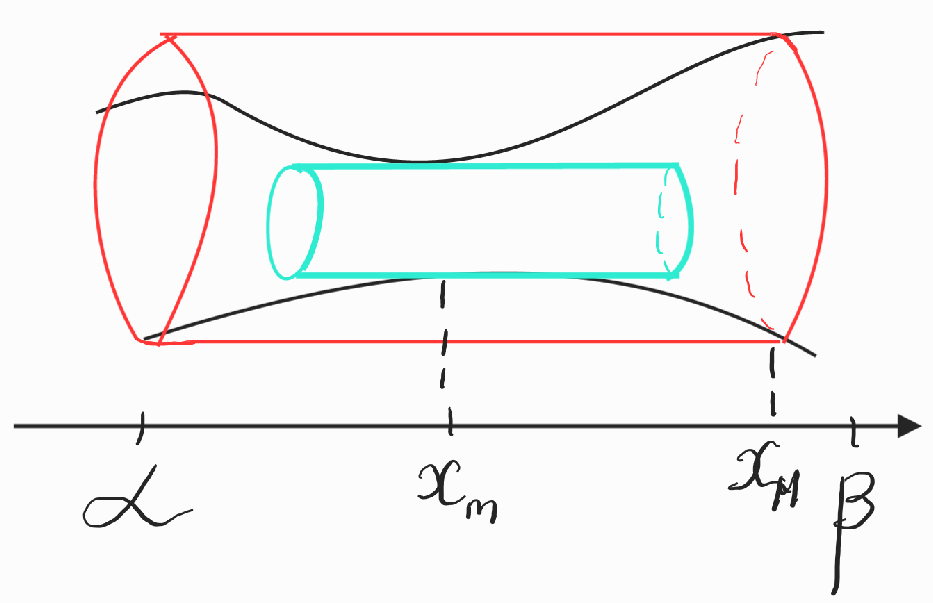
\includegraphics[width=\linewidth]{41_cylindr.pdf} 
        \end{minipage}
    }
    Условие длинное, но из него почти сразу получаем то, что хотим. Нужно через признак плотности сказать, что \( S\left( x\right)\) - плотность объёма, а для этого у нас почти всё есть. 

    Рассмотрим \( \Phi\left[ \alpha , \beta \right]=V\left( T \cap \left\{ \alpha \leq x \leq \beta \right\}\right),\quad \left[ \alpha , \beta \right] \subseteq \left[ a,b\right]\). \( \Phi\) - аддитивная функция промежутка, т.к. объём аддитивен (\hyperlink{thm:strong_monot}{\em{см. Усиленная монотонность}}). 
    \begin{equation*}
        \begin{aligned}
            &\left( T \cap \left\{ \alpha \leq x \leq \beta \right\}\right) \subseteq T\left( x_M,\cdot,\cdot\right)\times\left[ \alpha , \beta \right]\implies\\
            &V\left( T \cap \left\{ \alpha \leq x \leq \beta \right\}\right) \leq S\left( x_M\right)\left( \beta - \alpha \right) \leq \max\limits_{ \left[ \alpha , \beta \right]} S\cdot\left( \beta - \alpha \right)
        \end{aligned}
    \end{equation*}
    \[ \Phi\left[ \alpha , \beta \right] \leq \max\limits_{ \left[ \alpha , \beta \right]} S\left( x\right)\left( \beta- \alpha \right)\]
    \par Это можно представить на картинке: тело лежит внутри красного "цилиндра" (на самом деле это не совсем цилиндр, т.к. в основании не окружность, но так легче представлять).

    Аналогично \( \Phi\left[ \alpha , \beta \right] \geq S\left( x_m\right)\left( \beta- \alpha \right)\) (голубой "цилиндр" вписан в тело).
    
    Тогда по признаку плотности \( S\) - плотность \( \Phi\). 

    \[ \Phi\left[ a,b\right]=V\left( \underbrace{T \cap \left\{ x \in \left[ a,b\right],\quad y,z \in \R \right\}}_{T\text{, т.к. по условию }Pr_{Ox}\left( T\right)=\left[ a,b\right]}\right) = \displaystyle\int\limits_{ a}^{ b} S\left( x\right)dx\]

    \[ V\left( T\right)= \displaystyle\int\limits_{ a}^{ b} S\left( x\right)dx\]
\end{proof}

\begin{thm}[Объём тела вращения]\label{lab:thm:volume_rotation}

    ~

    \InsertBoxL{0}{
        \begin{minipage}[t]{6cm} 
            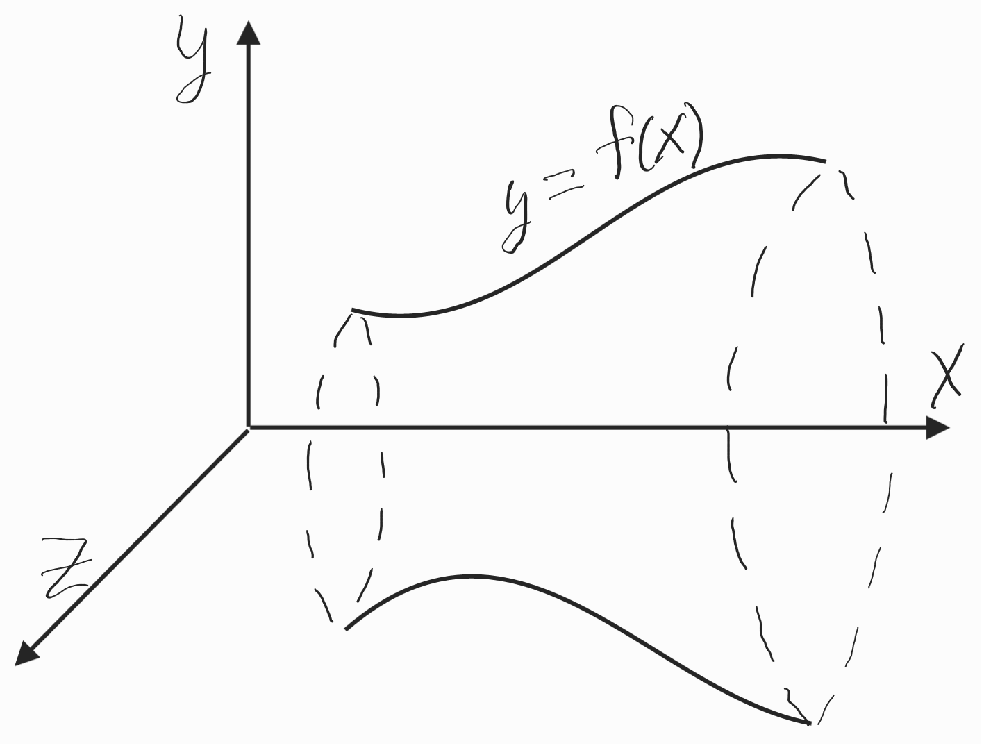
\includegraphics[width=\linewidth]{41_rotation.pdf} 
        \end{minipage}
    }

    \( \Let \; y=f\left( x\right),\quad f \in C\left[ a,b\right],\quad \forall \;x \in \left[ a,b\right] f\left( x\right) \geq 0\)

    Телом вращения называется множество 
    \[ T_{вр, Ox}=\left\{ \left( x,y,z\right):\; x \in \left[ a,b\right], \; y^2+z^2 \leq f^2\left( x\right)\right\}\]

    Тогда 
    \[ V\left( T\right)= \pi \displaystyle\int\limits_{ a}^{ b} f^2\left( x\right)dx\]
\end{thm}
\vspace{8pt}
\begin{proof}
    Это сразу получается из предыдущей теоремы. 

    Тело вращения удовлетворяет условию теоремы \ref{lab:thm:volume_via_section}, поэтому
    \[ V\left( T\right)= \displaystyle\int\limits_{ a}^{ b} S\left( T\left( x,\cdot,\cdot\right)\right)dx\]
    
    Но \( T\left( x,\cdot,\cdot\right)\) - это круг радиуса \( f\left( x\right) \implies S\left( T\left( x,\cdot,\cdot\right)\right)= \pi f^2\left( x\right)\)
    \[ V\left( T\right)= \displaystyle\int\limits_{ a}^{ b} \pi f^2\left( x\right)dx= \pi \displaystyle\int\limits_{ a}^{ b} f^2\left( x\right)dx\]
\end{proof}

\begin{example}[Объём \strike{арбуза} эллипсоида]
    
    ~

    \InsertBoxL{0}{
        \begin{minipage}[t]{6cm} 
            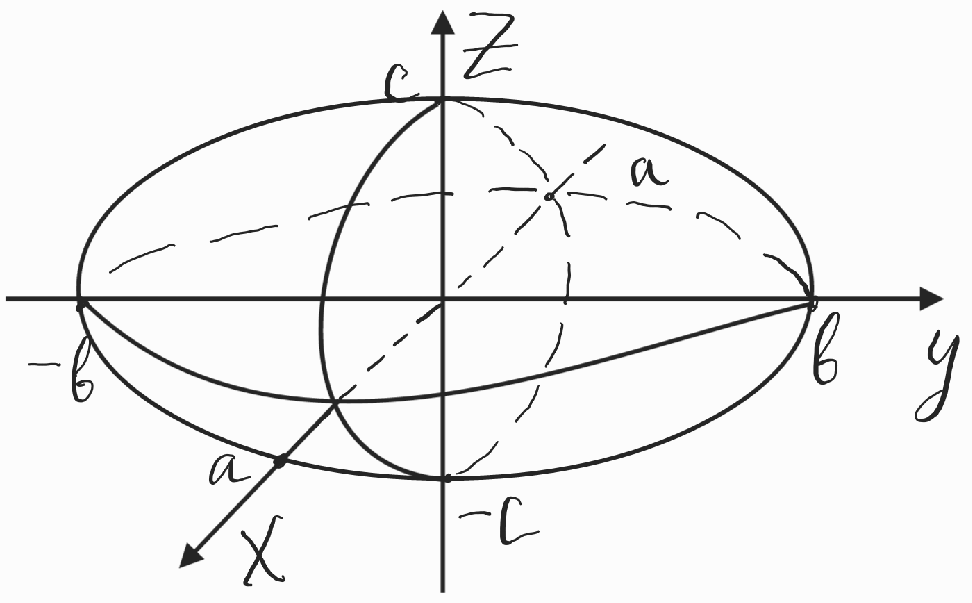
\includegraphics[width=\linewidth]{41_elipsoid.pdf} 
        \end{minipage}
    }

    Эллипсоид - это множество 
    \[ T=\left\{ \left( x,y,z\right):\quad \dfrac{ x^2}{ a^2}+ \dfrac{ y^2}{ b^2}+ \dfrac{ z^2}{ c^2} \leq 1\right\}\]

    Можно подумать, что эллипсоид - это тело вращения, но в случае различных
    \( a,b,c\) это неправда, поэтому считать его объём нужно через теорему \ref{lab:thm:volume_via_section}. 

    \[ T\left( x,\cdot,\cdot\right)=\left\{ \left( y,z\right):\; \dfrac{ y^2}{ b^2}+ \dfrac{ z^2}{ c^2} \leq 1- \dfrac{ x^2}{ a^2}\right\}\]

    \InsertBoxR{0}{
        \begin{minipage}[t]{6cm} 
            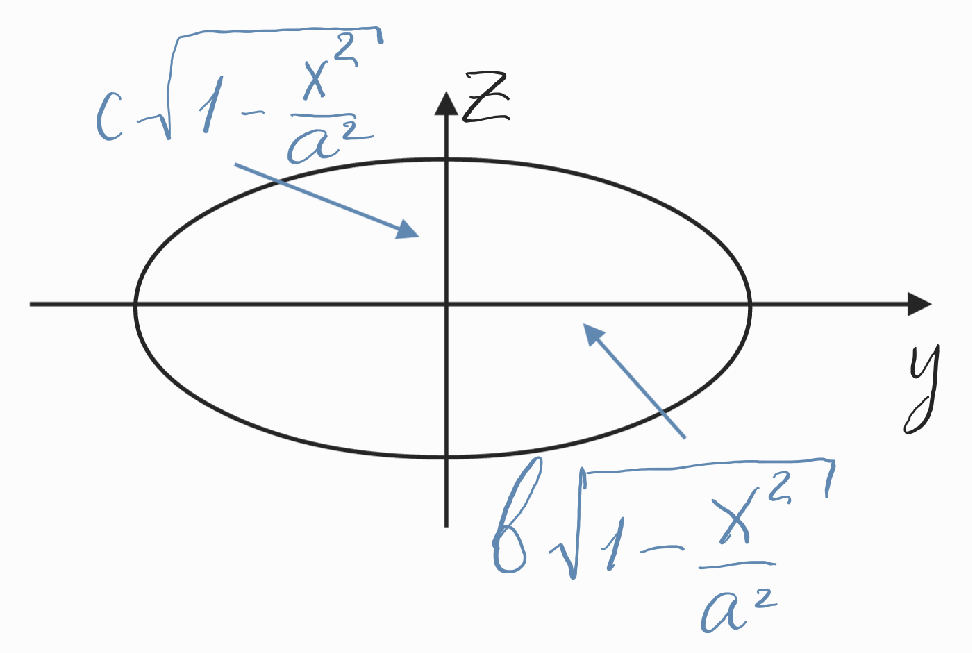
\includegraphics[width=\linewidth]{41_plain_elips.pdf} 
        \end{minipage}
    }

    \( T\left( x,\cdot,\cdot\right)\) - это эллипс, полуоси которого равны

    \[ c \;\sqrt[]{1- \dfrac{ x^2}{ a^2}} \text{ и } b \;\sqrt[]{1- \dfrac{ x^2}{ a^2}}\]

    \hyperlink{thm:elips_area}{Площадь эллипса мы умеем считать:}

    \[ S\left( x\right)= S\left( T\left( x,\cdot,\cdot\right)\right)= \pi bc\left( 1- \dfrac{ x^2}{ a^2}\right)\]
    \[ V\left( T\right)= \displaystyle\int\limits_{ -a}^{ a} S\left( x\right)dx=2 \pi bc \displaystyle\int\limits_{ 0}^{ a} \left( 1- \dfrac{ x^2}{ a^2}\right)dx \underset{t= \frac{ x}{ a}}{=}2 \pi bca \displaystyle\int\limits_{ 0}^{ 1} \left( 1-t^2\right)dt= \dfrac{ 4}{ 3} \pi abc\]
    \[ \boxed{V\left( T\right)= \dfrac{ 4}{ 3} \pi abc}\]
\end{example}

\begin{example}[Площадь пересечения цилиндров]

    ~

    Нужно найти объём множества
    \[ E=\left\{ \left( x,y,z\right):\;x^2+z^2 \leq a^2,\quad y^2+z^2 \leq a^2\right\}\]

    Рассмотрим сечение осью z:

    \[ E\left( \cdot,\cdot,z\right)=\left\{ \left( x, y\right):\;x^2 \leq a^2-z^2,\quad y^2 \leq a^2-z^2\right\}\]
    \begin{equation*}
        \begin{aligned}
            &x^2 \leq a^2-z^2\\
            &y^2 \leq a^2-z^2
        \end{aligned}
       \quad\Longleftrightarrow\quad 
       \begin{aligned}
            &\left| x\right| \leq \sqrt[]{a^2-z^2}\\
            &\left| y\right| \leq \sqrt[]{a^2-z^2}
       \end{aligned}
    \end{equation*}

    Таким образом, в сечении получается квадрат со стороной \( 2\;\sqrt[]{a^2-z^2}\). 

    \[ S\left( z\right)=4\left( a^2-z^2\right)\]

    И по теореме \ref{lab:thm:volume_via_section}:

    \[ V\left( E\right)= \displaystyle\int\limits_{ -a}^{ a} S\left( z\right)dz=2\cdot4 \displaystyle\int\limits_{ 0}^{ a} \left( a^2-z^2\right)dz= \dfrac{ 16}{ 3}a^3\]

    \[ \boxed{V\left( E\right)= \dfrac{ 16}{ 3} a^3}\]
\end{example}

\begin{example}[Объём полнотория]
    
    ~

    \InsertBoxL{0}{
        \begin{minipage}[t]{6cm} 
            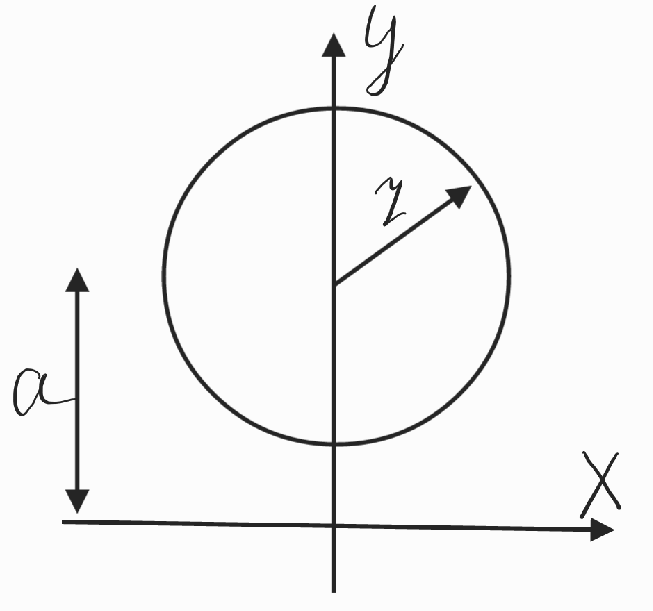
\includegraphics[width=\linewidth]{41_tor.pdf} 
        \end{minipage}
    }

    Этого не было в лекции, но почему бы не посчитать. Полноторий - это множество \( T\), ограниченное тором. Тор - это поверхность, полученная вращением окружности вокруг оси \( x\).
    Таким образом, полноторий - тело вращения и считать его объём мы будем по теореме \ref{lab:thm:volume_rotation}. 
    
    Пусть окружность задана уравнением 
    \[ x^2+\left( y-a\right)^2=r^2 \implies y=\pm\; \sqrt[]{r^2-x^2}+a\]

    \vspace{6pt}
    \begin{flushleft}
        \begin{equation*}
            \begin{aligned}
                &V\left( T\right)= \pi \displaystyle\int\limits_{ -r}^{ r} \left( \; \sqrt[]{r^2-x^2}+a\right)^2dx- \pi \displaystyle\int\limits_{ -r}^{ r} \left( -\; \sqrt[]{r^2-x^2}+a\right)^2dx= \\ 
                &=4\pi a \displaystyle\int\limits_{ -r}^{ r} \; \sqrt[]{r^2-x^2}dx \underset{t=r\sin x}{=}4 \pi a \displaystyle\int\limits_{ - \frac{ \pi}{ 2}}^{ \frac{ \pi}{ 2}} r^2\cos^2 t\;dt=2 \pi^2 a r^2
            \end{aligned}
        \end{equation*}
    \end{flushleft}
    \[ \boxed{V\left( T\right)=2 \pi^2 ar^2}\]
\end{example}
\end{document}